\thispagestyle{empty}
\newpage
\begin{flushleft}
\textbf{Транзитивные множества}

\textbf{и правильные многогранники}

\textit{(см. \guillemotleft Квант\guillemotright № 7)}
\end{flushleft}
\begin{center}
    \textbf{Параметры правильных многогранников}
\end{center}
\begin{left}
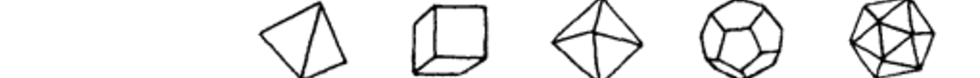
\includegraphics[\textwidth]{ris1}
%\caption{Рис. 1}
\end{left}
\begin{center}
\renewcommand{\arraystretch}{2}
\begin{tabular}{ | m{11em} | >{\centering\arraybackslash} m{2.2cm} | >{\centering\arraybackslash} m{2.2cm} | >{\centering\arraybackslash} m{2.2cm} | >{\centering\arraybackslash} m{2.2cm} | >{\centering\arraybackslash} m{2.2cm} | } 
 \hline
 & Тетраэдр & Куб & Октаэдр & Додекаэдр & Икосаэдр \\
 \hline
 Число граней & 4 & 6 & 8 & 12 & 20  \\
 \hline
 Число вершин & 4 & 8 & 6 & 20 & 12  \\
 \hline
 Число ребер & 6 & 12 & 12 & 30 & 30  \\
 \hline
 Косинус угла, под которым ребро видно из центра опис. сферы & $-\frac{1}{3}$ & $\frac{1}{3}$ & 0 & $\frac{\sqrt{5}}{3}$ & $\frac{1}{\sqrt{5}}$  \\
 \hline
 Косинус двугранного угла & $\frac{1}{3}$ & 0 & $-\frac{1}{3}$ & $-\frac{1}{\sqrt{5}}$ & $-\frac{\sqrt{5}}{3}$  \\
 \hline
 Радиус опис. сферы & $\frac{a\sqrt{3}}{2\sqrt{2}}$ & $\frac{a\sqrt{3}}{2}$ & $\frac{a}{\sqrt{2}}$ & $\frac{a\xi\sqrt{3}}{2}$ & $\frac{a\sqrt{\xi}\sqrt[4]{5}}{2}$  \\
 \hline
 Радиус впис. сферы & $\frac{a}{2\sqrt{6}}$ & $\frac{a}{2}$ & $\frac{a}{\sqrt{6}}$ & $\frac{a\sqrt{\xi^3}}{2\sqrt[4]{5}}$ & $\frac{a\sqrt{\xi^3}}{2\sqrt{3}}$  \\
 \hline
Площадь поверхности & $a^2\sqrt{3}$ & $6a^2$ & $2a^2\sqrt{3}$ & $\frac{15a^2\sqrt{\xi^3}}{\sqrt[4]{5}}$ & $5a^2\sqrt{3}$  \\
\hline
Объем & $\frac{a^3}{6\sqrt{2}}$ & $a^3$ & $\frac{a^3\sqrt{2}}{3}$ & $\frac{a^3\xi^4\sqrt{5}}{2}$ & $\frac{5a^3\sqrt{\xi^3}}{6}$  \\
\hline
\end{tabular}
\end{center}
\setlength{\parindent}{0pt}
\begin{left}
\noindent\text{(\emph{a} "--- длина ребра; через $\xi$ обозначено число $\frac{1+\sqrt{5}}{2}\approx1,618045$)}
\end{left}

\begin{multicols}{2}
\textbf{Несколько вопросов по астрономии}

\textit{(см. \guillemotleft Квант\guillemotright № 5. с. 42)}

\textbf{1.} В любой точке экватора продолжительность дня равна продолжительности ночи.

\textbf{2.} Смена времен года на экваторе существует. Хотя Солнце находится над горизонтом всегда ровно 12 часов, его максимальная высота над горизонтом день ото дня изменяется. 

\textbf{3.} На экваторе два раза в год --- в дни весеннего (21 марта) и осеннего (23 сентября) равноденствий --- Солнце в поледнь бывает в зените. Таким образом, самые жаркие дни на экваторе приходятся на весну и на осень. В то время как в средних широтах за год происходит один цикл смены времен года, на экваторе происходят два таких цикла. 

\textbf{4.} Нет, не промежуточная. На экваторе в день летнего солнцестояния (впрочем, как и в день зимнего солнцестояния) высота кульминации Солнца наименьшая по сравнению с другими днями в году.\\
\vspace{6cm}

\hline
\textit{Номер готовили:} \\
А.~Виленкин, А.~Егоров, И.~Клумова, Т.~ Петрова, \\
А.~Сосинский, В.~Тихомирова, Ю.~Шиханович \\
\hline
\textit{Номер оформили:} \\
К.~Борисов, М.~ Дубах, Г.~Красиков, Э.~Назаров,\\
А.~Пономарева
\hline
\emph{Зав.~редакцией} Л.~Чернова \\
\hline 
\emph{Художественный редактор} Г.~Макарова \\
\hline
\emph{Корректор} О.~Кривенко \\
\hline
113055 Москва, М-35, Б. Ордынка, 21/16, \\
\guillemotleft Квант\guillemotright. тел. 231-83-62 \\
Сдано в набор 17.VI-80.\\
Подписано в печать 17.VII-80. \\
Печать офсетная \\
Бумага $70\times108$ 1/16. Физ. печ. л. 4. \\
Усл. печ. л. 5,6. Уч. изд. л. 7.43\\
Цена 30 коп. Заказ 1400.\\
Тираж 260311 экз.
\hline
Чеховский полиграфический комбинат \\
Союзполиграфпрома\\
Государсвтенного комитета \\
СССР по делам издательства, полиграфии \\
и книжной торговли. \\
г.~Чехов Московской области\\
\hline
\end{multicols}
\newgeometry{left=0.8cm,right=0.8cm,bottom=0.1cm,top=2cm}
\thispagestyle{fancy}
\fancyhead{} 
\fancyhead[C]{\Large ФОРМУЛЫ}
\begin{center}
\[corr(\emph{X,Y})=\frac{\displaystyle\sum_{i=1}^{n}(x_i-\bar x)(y_i-\bar y)}{\biggl[\displaystyle\sum_{i=1}^{n}(x_i-\bar x)^2\displaystyle\sum_{i=1}^{n}(y_i- \bar y_2)^2\biggr]^\frac{1}{2}}\]\\
\[
\sin{x} = \frac{2\tg{\frac{x}{2}}}{1+\tg^2{\frac{x}{2}}}
\]
\[\sin^6(x) + \cos^6(x)=(sin^2(x)+cos^2(x))(sin^4(x)-sin^2(x)cos^2(x)+cos^4(x))=1-3sin^2(x)cos^2(x)\]\\
\[\text{Высокий порядок производных: }
\frac{d^nf(x)}{dx^n}=\displaystyle\sum_{k=0}^nS(n,k)f^{(k)}(x)\frac{x^k}{k!}
\]
\[\text{Разложение Фурье: }
f(x)=a_0 + \displaystyle\sum_{n=1}^{\infty}((\frac{1}{\pi}\int_{-\pi}^{\pi}f(x)\cos{(nx)}dx)\cos{(nx)}+(\frac{1}{\pi}\int_{-\pi}^{\pi}f(x)\sin{(nx)}dx)\sin{(nx)}
\]\\
\[\text{Формула для исследования эффекта размывания}X_k = \frac{A}{2}\biggl[ e^{j\phi}\frac{e^{2\pi j(n-k)}e^{2\pi jq}-1}{e^{\frac{2\pi j(n+q-k)}{N}-1}}+e^{-j\phi}\frac{e^{-2\pi j(n+k)}e^{-2\pi jq}-1}{e^{\frac{e^{-2\pi j(n+q+k)}}{N}}-1}\biggr]
\]
\end{center}
